\documentclass[../main.tex]{subfiles}

\begin{document}
In this section, some results from the implementation of the approach described in \ref{sec:SolutionArchitecture} will be shown. The inverted pendulum system has been modelled as a MDP with $x_1\in [-\frac{\pi}{2}, \frac{\pi}{2}] $ and $x_2 \in [-5\, \frac{\text{rad}}{s},5 \,\frac{\text{rad}}{s}] $. The state space has been discretised with $19$ steps in both dimensions and the action space has been discretised with $5$ steps on the range $u \in [-25\,\text{N},25\,\text{N}] $. The time step for the learning loop is chosen as $h_\text{learn} = 0.2\text{ s}$ and $h_\text{safe} = 0.005\,\text{s}$. The true disturbance introduced to the system is chosen to be $d = 0.5\sin(5x_1)$ and initially bounded conservatively with $\overline{d}_0 = 10 \,\text{N}$ and $\underline{d}_0 = -10 \,\text{N}$. The safe region $\mathcal{S}_0$ is a rectangle centered around the origin with width $0.9\pi$ in $x_1$-direction and width $10\frac{\text{rad}}{s}$ in $x_2$-direction. In each iteration the set is calculated for $\tau = 40\,\text{s}$.

In the following, the results from four learning iterations at each $10,000$ steps will be presented. After each iteration a new disturbance estimation and safe set calculation is done. As described in Section \ref{sec:Exploration}, it is crucial for the disturbance and policy estimation that all states within the safe set have been visited sufficiently often. A method for structured exploration, Incremental Q-learning, has been introduced. In this section, the results from incorporating exploration will be compared to those yielded from the approach without structured exploration. 

To begin with, we look at the distribution of $1000$ random samples drawn from the recorded samples of all four iterations. Figure \ref{fig:samples_exploration} shows the sampling results of the algorithm with exploration compared to the one without exploration. 

\begin{figure}
    \centering
    \begin{subfigure}[b]{\textwidth}
    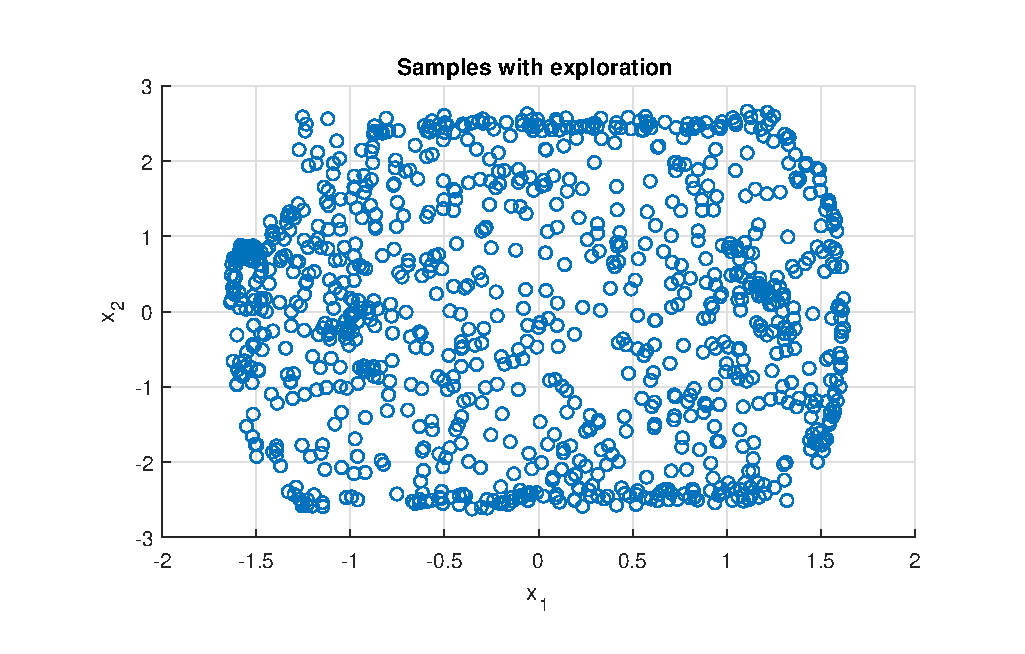
\includegraphics[width=\textwidth]{samples_exploration}
    \end{subfigure}
    
    \begin{subfigure}[b]{\textwidth}
    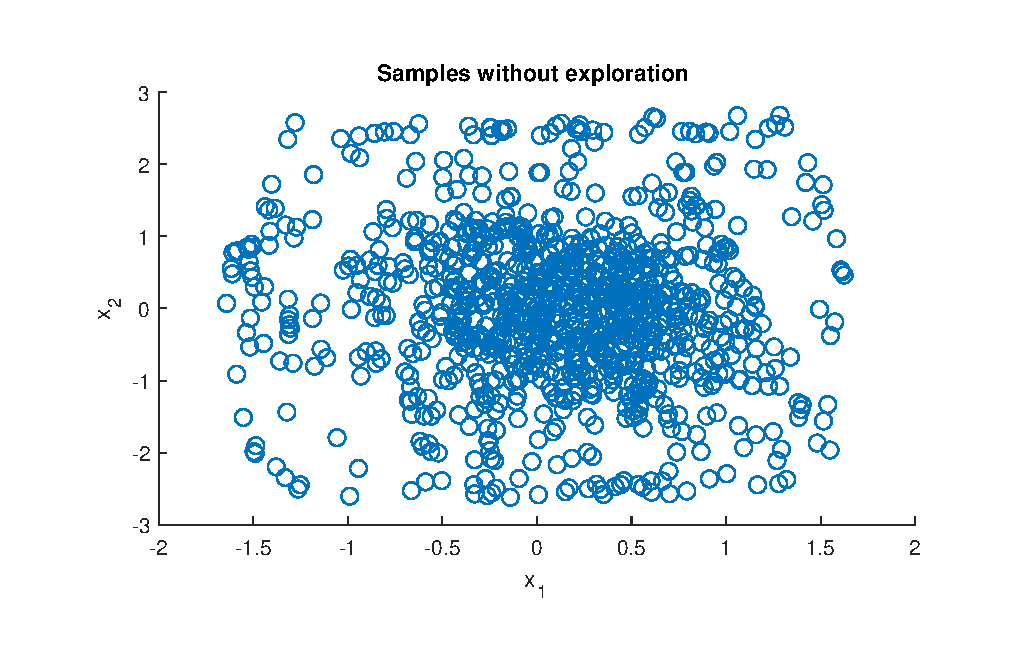
\includegraphics[width=\textwidth]{samples_unexploration}
    \end{subfigure}
        \caption{Random sampling with and without Incremental Q-learning. In the upper figure, the spread of the samples is clearly better, whereas in the lower figure most samples are concentrated around the origin.}  \label{fig:samples_exploration}
\end{figure}

It can clearly be seen that the samples are a lot more wide-spread, if exploration is done. Without exploration, the learning algorithm always decides for the action that is most promising in order to keep the system close to the origin. This causes a concentration of samples around this point that might inhibit both the disturbance estimation and the policy learning at the edges of the safe set. 

It is therefore interesting to compare, if Incremental Q-learning as described in Section \ref{sec:Exploration} yields a better estimation of the policy. The results of this comparison are depicted in Figure \ref{fig:policy_exploration}. The figure shows the estimated policy from each state, where the respective colors correspond to values of $u$. Because the action values are not really decisive, it has been decided to not show a legend that matches colors to values. Instead, the quality of the estimated policy can be decided upon by comparing to the optimal policy that has been found with Policy Iteration (left figure). Clearly, the results are better for the approach that incorporates exploration. This can especially seen at the edges of the safe set where the estimated policy without exploration is very inaccurate (right figure).

\begin{figure}
    \centering
    \makebox[\textwidth][c]{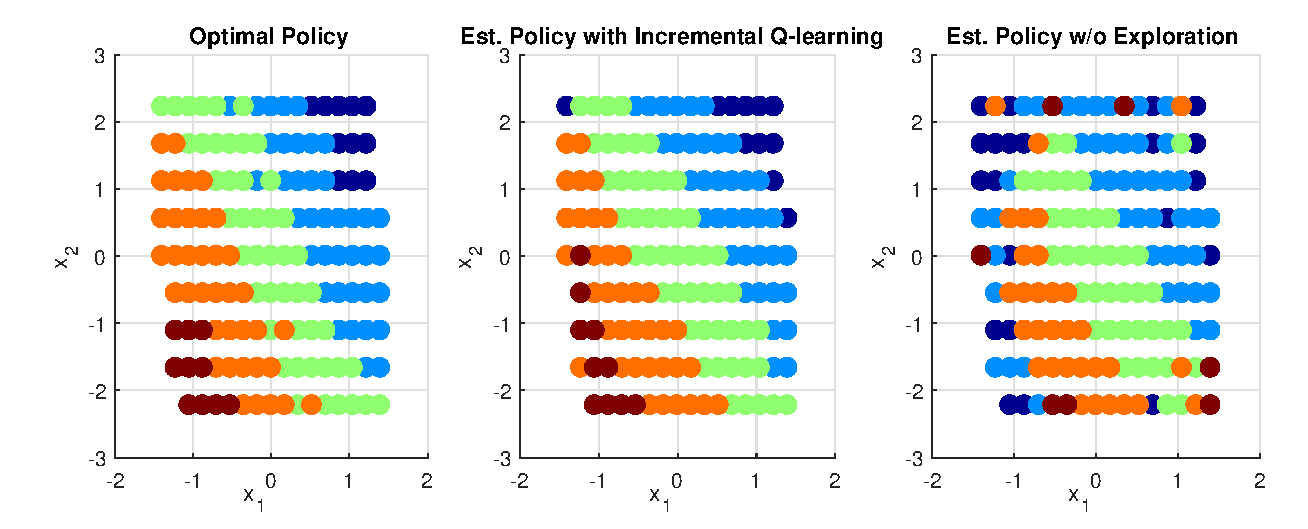
\includegraphics[width=1.2\textwidth]{policy_exploration}}
    \caption{Policy estimated with and without exploration. After the same number of learning iterations, the algorithm with exploration achieves considerably better results above all at the edges of the safe set.} \label{fig:policy_exploration}
\end{figure}

To quantify the findings from Figure \ref{fig:policy_exploration}, the absolute error between the estimated and the optimal policy is illustrated in \ref{fig:PolicyError}. In addition to the algorithm without exploration and with Incremental Q-learning, the error with $\epsilon$-greedy exploration is shown. It can be seen that the Incremental Q-learning approach takes slightly longer to converge but achieves a remarkably better result. It becomes also clear that the deterministic approach to exploration, Incremental Q-learning, pays off in comparison to the randomized $\epsilon$-greedy exploration. 

\begin{figure}[h]
    \centering
    \makebox[\textwidth][c]{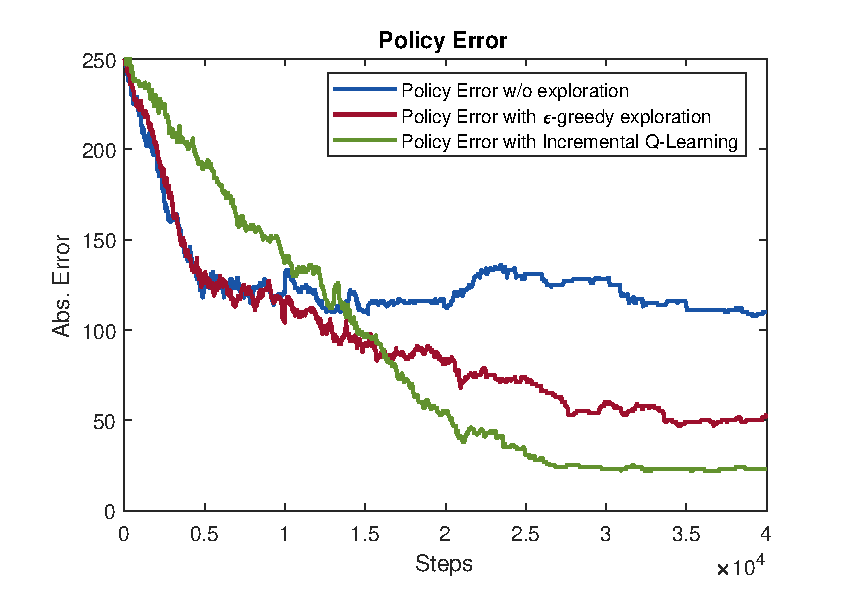
\includegraphics[width=\textwidth]{PolicyError}}
    \caption{Policy error with Incremental Q-learning, $\epsilon$-greedy eploration and without exploration. The approach with Incremental Q-learning converges slightly slower but the final error without exploration is about four times higher than the error of the Incremental Q-learning algorithm.} \label{fig:PolicyError}
\end{figure}

However, on the long run, pure exploration might not be the most desirable strategy. After all states have been visited sufficiently often, one would wish to exploit the most promising strategy. In the present system, this means that after sufficient exploration one would wish to keep the pendulum stable around the origin. This can be for example be realized by switching off the exploration after all states have been visited $100$ times. It is therefore interesting to investigate if the exploration algorithm can guarantee that all states are visited a sufficient number of times. Figure \ref{fig:leastvisited} shows the number of visits of the ten least visited states with and without exploration. 
\begin{figure}[h]
    \centering
    \makebox[\textwidth][c]{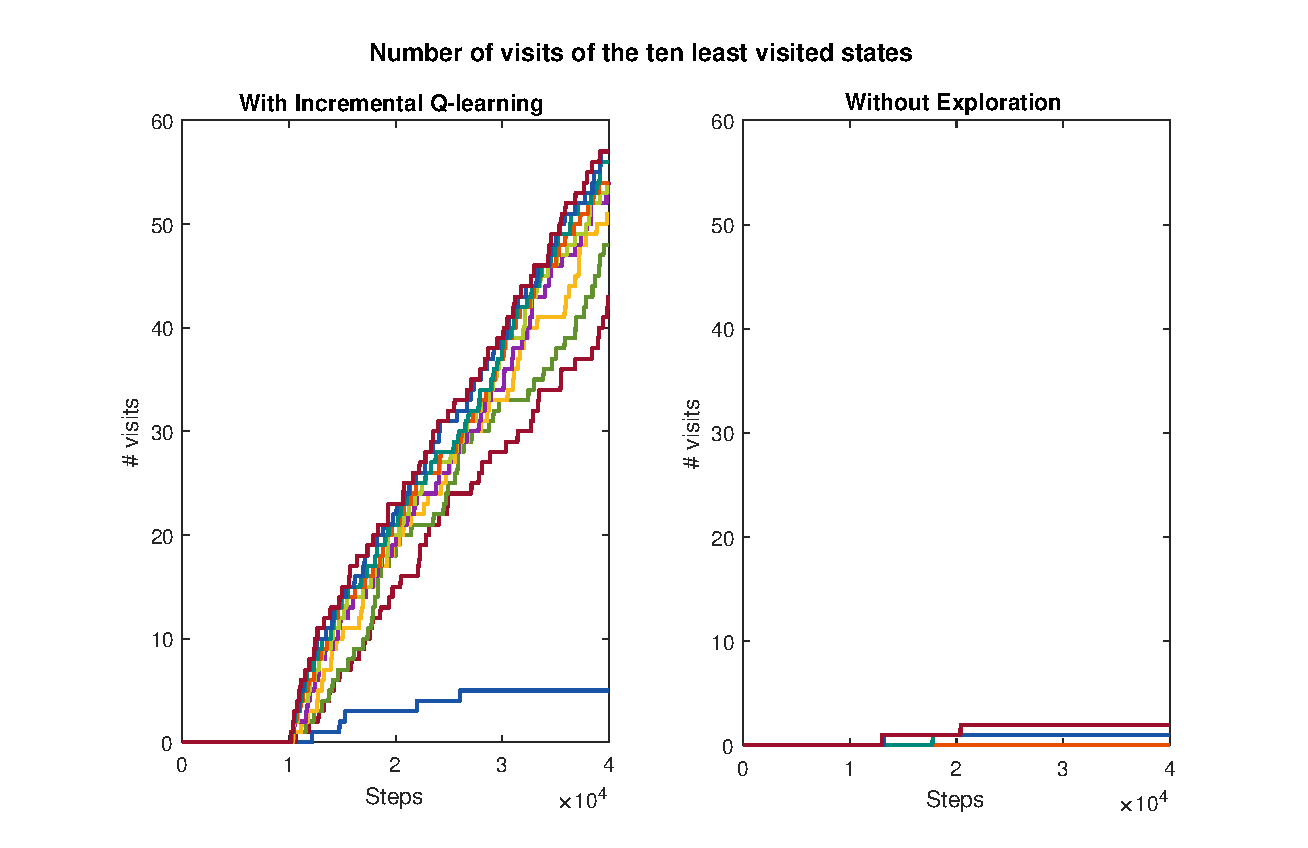
\includegraphics[width=\textwidth]{leastvisited}}
        \caption{Number of visits of the ten least visited states with and without exploration respectively.}  \label{fig:leastvisited}
\end{figure}
Without exploration, several states remain unvisited for all $40,000$ steps. None of the ten least visited state gets visited more than ten times. With exploration, the system passes all states within the first $20,000$ steps. Except from one, all states count more than $40$ visits within the observed $40,000$ steps. This indicates that it might indeed be possible to switch off the Incremental Q-learning after a certain number of iterations. A suitable criteria could be identified by examining the policy error of a state in proportion to the number of visits. The number of visits that is sufficient to eliminate the error could serve as bound for how often all states need to be visited until exploration can be switched off. This promising variant of the algorithm has however not been implemented in the present work.\par

In the following, the influence of exploration on the disturbance estimation will be examined. Figure \ref{fig:GP_it4_doubleexplore} shows the result from the disturbance estimation with Gaussian Process regression after each iteration with the above described setup. The left half of the figure shows the result from the approach without exploration. The right half shows the results with Incremental Q-learning. For both algorithms it can be seen that the disturbance estimation gets better with each iteration. This is caused by the fact that the system visits wider regions of the state space with an increasing number of steps. Therefore, the samples taken from the recorded data points are spread out wider the more steps are recorded. Furthermore, it becomes clear that the disturbance estimation indeed is better for the approach with exploration. In the results without exploration, the samples are more concentrated in the front half of the coordinate system so that the disturbance estimate is good in that region but almost constant in the rear half and outside the safe set. In the results with exploration, the sinusoidal shape of the disturbance is clearly visible from the third iteration onwards. The disturbance estimate is quite accurate for all states within the safe set. 

\begin{figure}[H]
    \centering
    \makebox[\textwidth][c]{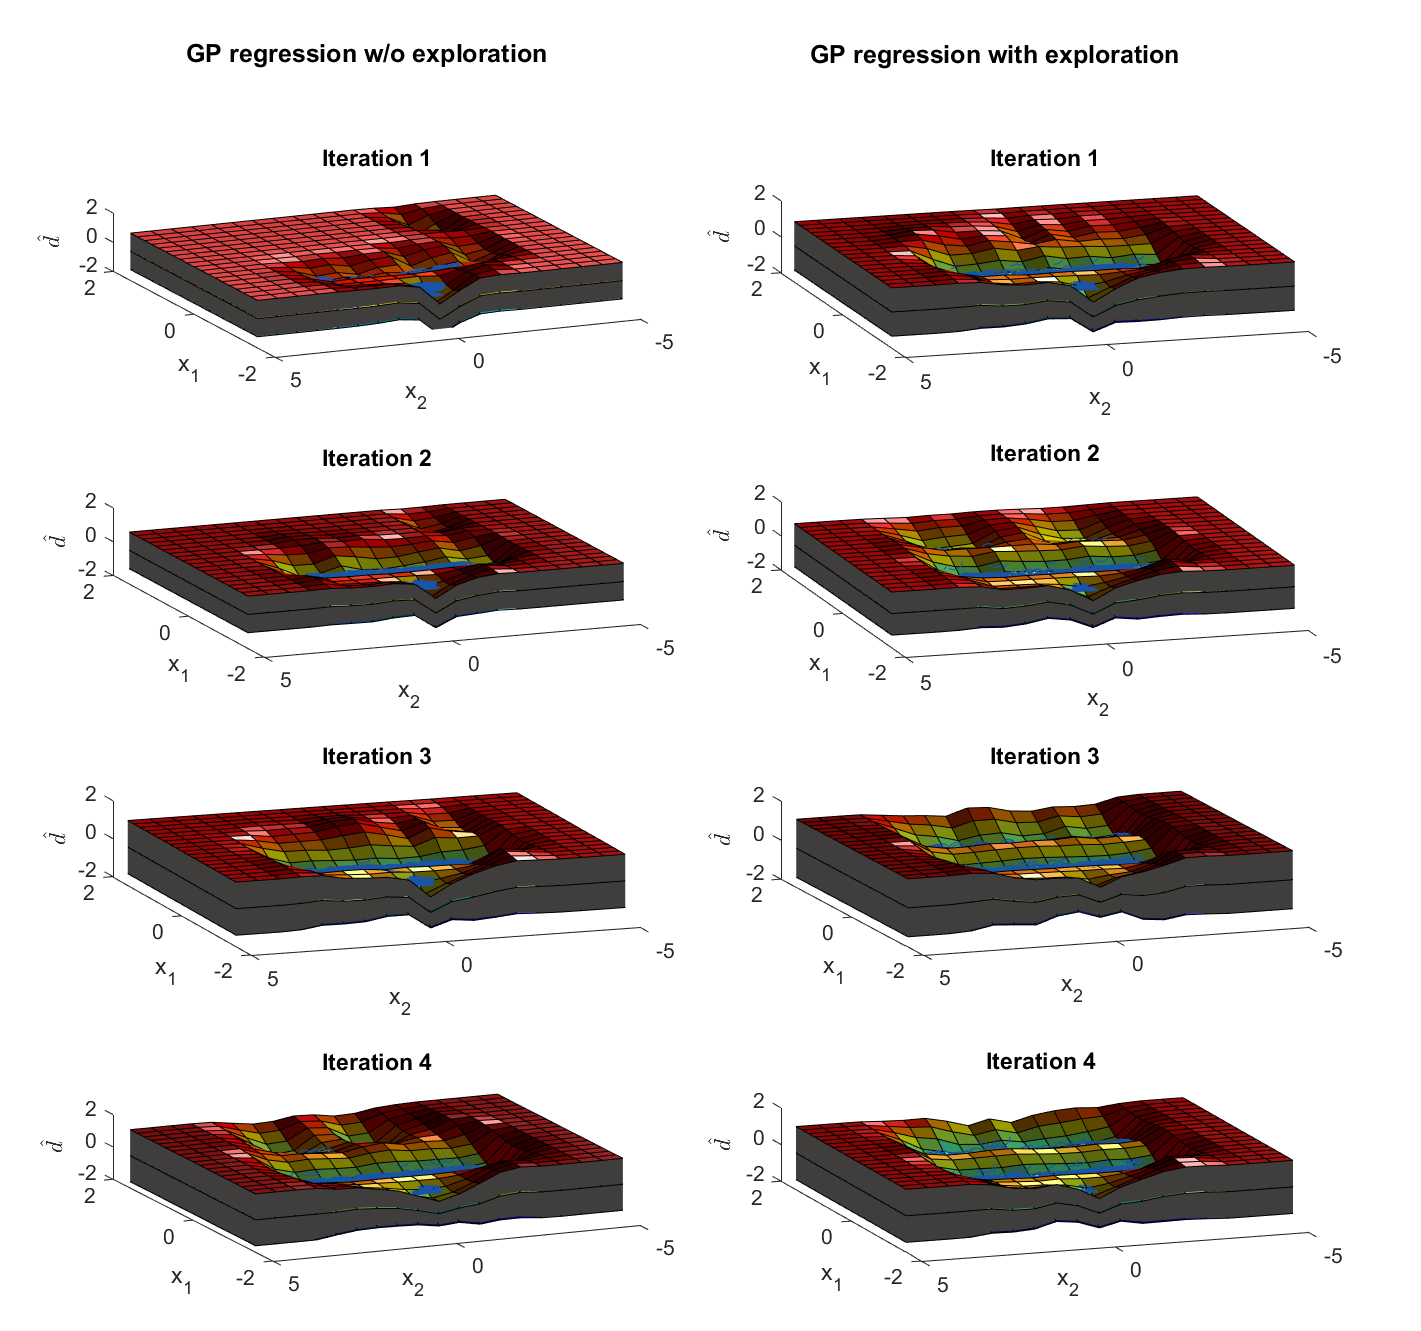
\includegraphics[width=1.2\textwidth]{GP_it4_doubleexplore}}
        \caption{Gaussian Process regression in four iterations.}  \label{fig:GP_it4_doubleexplore}
\end{figure}


Figure \ref{fig:SafeSet_it4_unexplore} shows the safe set computations for all four iterations. During the first iteration, the conservative initial bound is used for the safe set calculations and gives a relatively small initial safe set. By calculating a better disturbance estimate in the Gaussian Process regression, the safe set grows already largely in the second iteration. 
\begin{figure}[h]
    \centering
    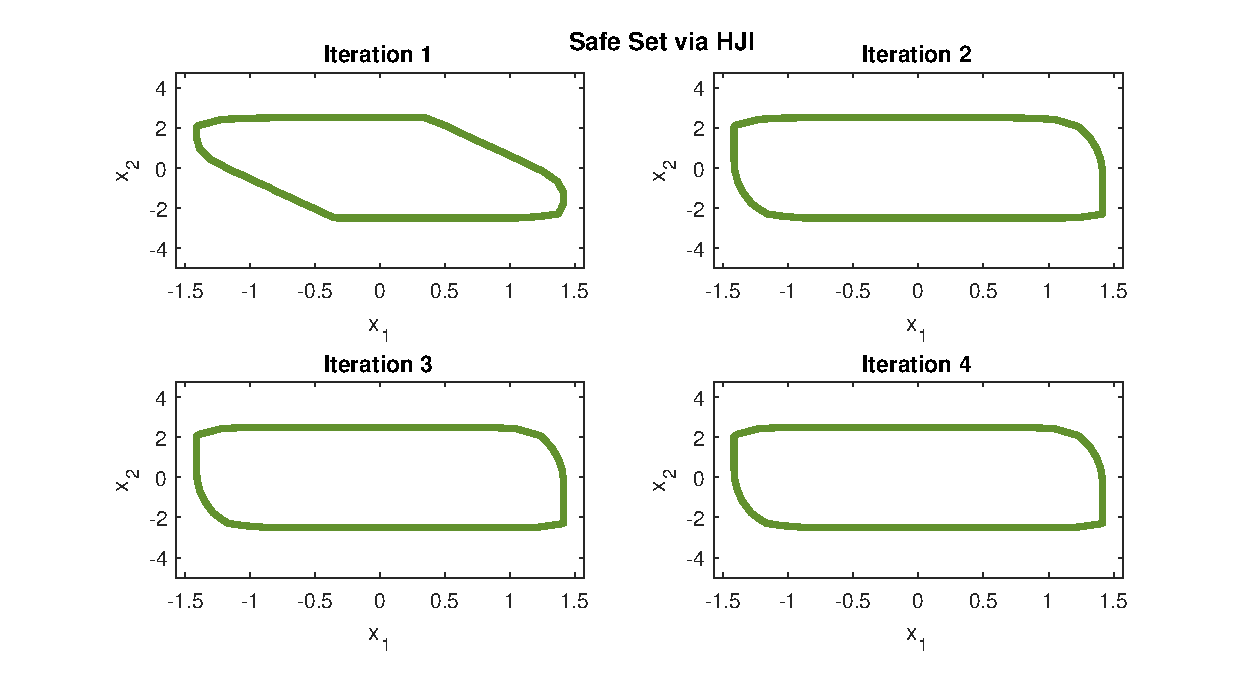
\includegraphics[width=\textwidth]{SafeSet_it4_unexplore}
        \caption{Safe set computation in four iterations. The better disturbance estimate causes an increase in the safe states already after the first iteration.}  \label{fig:SafeSet_it4_unexplore}
\end{figure}

Interestingly, the safe set resulting from the disturbance estimate is the same without and with exploration. The result for all four iterations can be seen in Figure \ref{fig:SafeSet_it4_unexplore}. After the first iteration the safe set increases due to the improved estimate. From the second iteration onwards, the set remains the same. A reason for this behaviour might be that the safe set is a over-approximation of the true safe set that not necessarily increases as the disturbance bounds decrease. This claim gets supported by the fact that the safe set remains the same even if a disturbance of $d = 0\,\text{N}$ is assumed.\par

Finally, simulation results from both approaches are portrayed in Figure \ref{fig:Simulation}. The depicted trajectories show the last $500,000$ samples that have been recorded with $h_\text{safe} = 0.005\,\text{s}$. It becomes clear that the algorithm with exploration causes the system to explore the whole state space and repeatedly hit the borders of the safe set. The approach without exploration manages to keep the system close to the origin. 

\begin{figure}
    \centering
    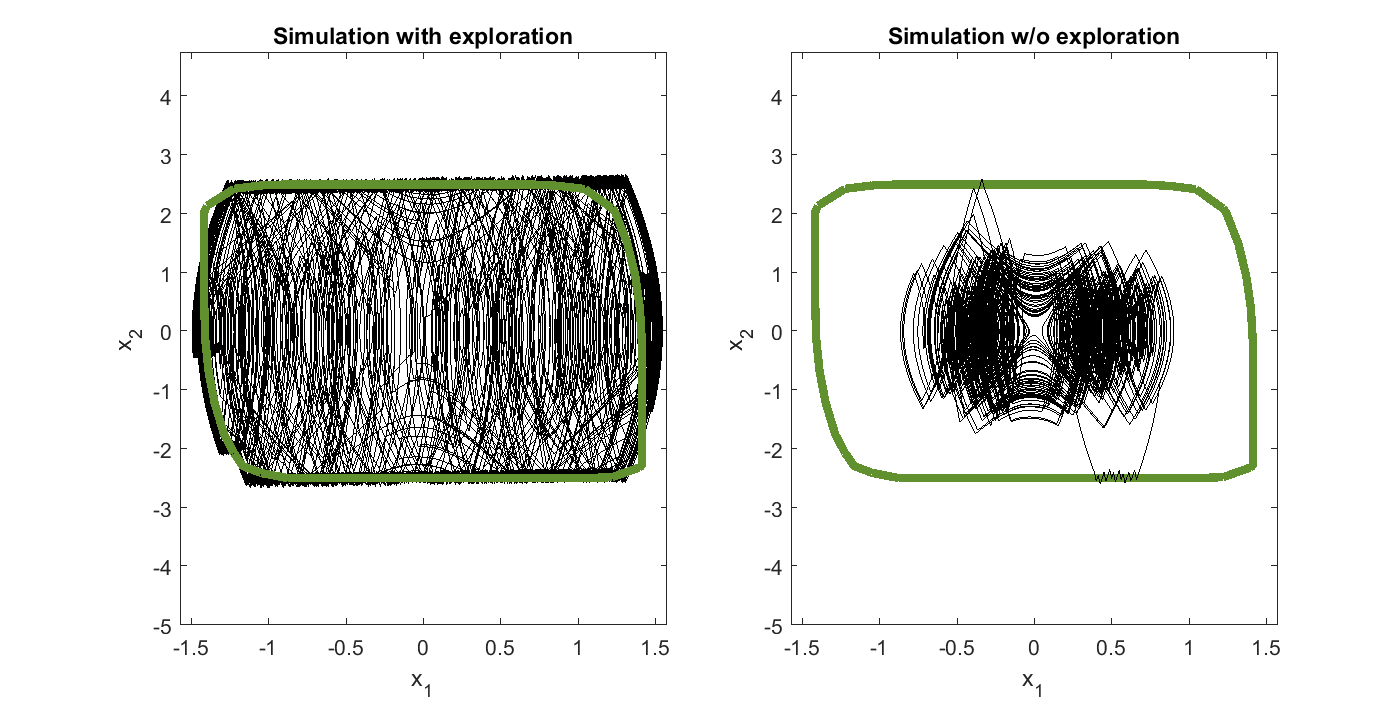
\includegraphics[width=\textwidth]{Simulation}
        \caption{Simulation of the system with Incremental Q-learning versus simulation without exploration.}\label{fig:Simulation}
\end{figure}

\end{document}
